\chapter{Mediciones y Resultados}
This chapter will summarize the measurements made and the results obtained after the development of the biosensors. It will be divided into three procedures differentiated by the type of characterization: electrical, dimensional and electrochemical.

\section{Caracterización eléctrica}
Four-point resistance measurements were made obtaining the following results:

$\bullet$ Between two carbon pads: \textbf{2,2 k$\Omega$}.

$\bullet$ Same carbon pads with a layer of cured gold nanoparticles ink: \textbf{1,15 k$\Omega$}.

$\bullet$ Same carbon pads with two layers of cured gold nanoparticles ink: \textbf{500 $\Omega$}.

Given the deposition of the gold ink layer on the carbon, a parallel is formed between the two elements. Using the equation of resistors in parallel (\ref{ecuacion1}), the resistance of the one and two cured layers of gold nanoparticles can be calculated.

\begin{equation}\label{ecuacion1}
R_{1//2}=\frac{R_{1} \times R_{2}}{R_{1}+R_{2}}
\end{equation}

De esta forma se obtienen los siguientes valores:

$\bullet$ A layer of cured gold nanoparticles: \textbf{2,4 k$\Omega$}.

$\bullet$ Two layers of cured gold nanoparticles: \textbf{0,65 $\Omega$}.

Assuming that the gold layers are thin film prints, the equation (\ref{ecuacion2}) is used to obtain the resistivity of the material,

\begin{equation}\label{ecuacion2}
\rho_{Bulk}=\frac{R \times w \times t}{L}
\end{equation}

where $\rho$\textsubscript{Bulk} is the resistivity, $R$ the resistance, $w$ the width, $t$ the thickness and $L$ the length of the material. In this case, the gold nanoparticles path. The width of the design is 0.04 cm, the average thickness for two layers 0.00055 cm (obtained by profilometer) and the length 1.05 cm giving the following results:

$\bullet$ A layer of cured gold nanoparticles ink (assuming half the thickness): \textbf{0,025 $\Omega$ $\times$ cm}

$\bullet$ Two layers of cured gold nanoparticles ink: \textbf{0,0000136 $\Omega$ $\times$ cm o 13,6 $\mu\Omega$ $\times$ cm}

According to the materials resistivity table, pure gold has a resistivity of \textbf{2,35 $\mu\Omega$ $\times$ cm} \cite{Resistividad}.

\section{Dimensional characterization}
After optically measuring the eight electrodes in a cartridge, the diameter was averaged at \textbf{993 $\mu$m} and the separations between elements of the electrochemical cell at \textbf{390 $\mu$m}.

The table of the figure~\ref{fig:Figura_tabla_rugosidades} shows the results of the roughness obtained.

\begin{figure}[H]
  \centering
    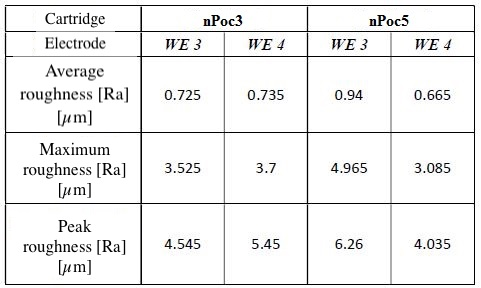
\includegraphics[width=0.6\textwidth]{Figures/Figura_tabla_rugosidades}
  \caption{Roughness values obtained for two \emph{WE} from two biosensors (nPoc3 and nPoc5).}
  \label{fig:Figura_tabla_rugosidades}
\end{figure}

The thicknesses of the same \emph{WE} were measured on the same biosensors. In order to obtain the estimated thickness of the 2 layers printed with the gold nanoparticles ink, the thickness was measured on a pure carbon electrode.

The table of the figure~\ref{fig:Figura_tabla_espesores} shows the values obtained from the thicknesses.

\begin{figure}[H]
  \centering
    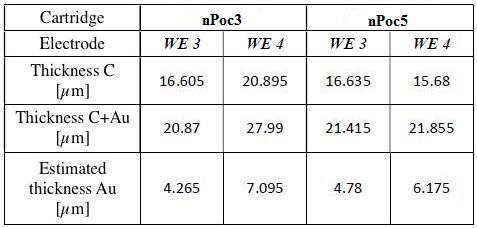
\includegraphics[width=0.6\textwidth]{Figures/Figura_tabla_espesores}
  \caption{Thickness values obtained for two \emph{WE} of two biosensors (nPoc3 and nPoc5).}
  \label{fig:Figura_tabla_espesores}
\end{figure}

The tables were extracted from the report made at the Center for Physics and Metrology of the National Institute of Industrial Technology \cite{caracdimen}.

\section{Caracterización electroquímica}
The first cyclic voltammetry was performed with a pure gold electrode deposited on silicon using a \textit{Sputtering} process. The response for the ferro and ferricyanide electrochemical probes on a \textit{sputtering} deposited gold electrode was obtained (Figure ~\ref{fig:Figura_EQ_Oro_Sputtering_1mm}), which will be used as a reference to compare with electrodes printed with gold nanoparticles ink using the \textit{Inkjet} printing process.

\begin{figure}[H]
  \centering
    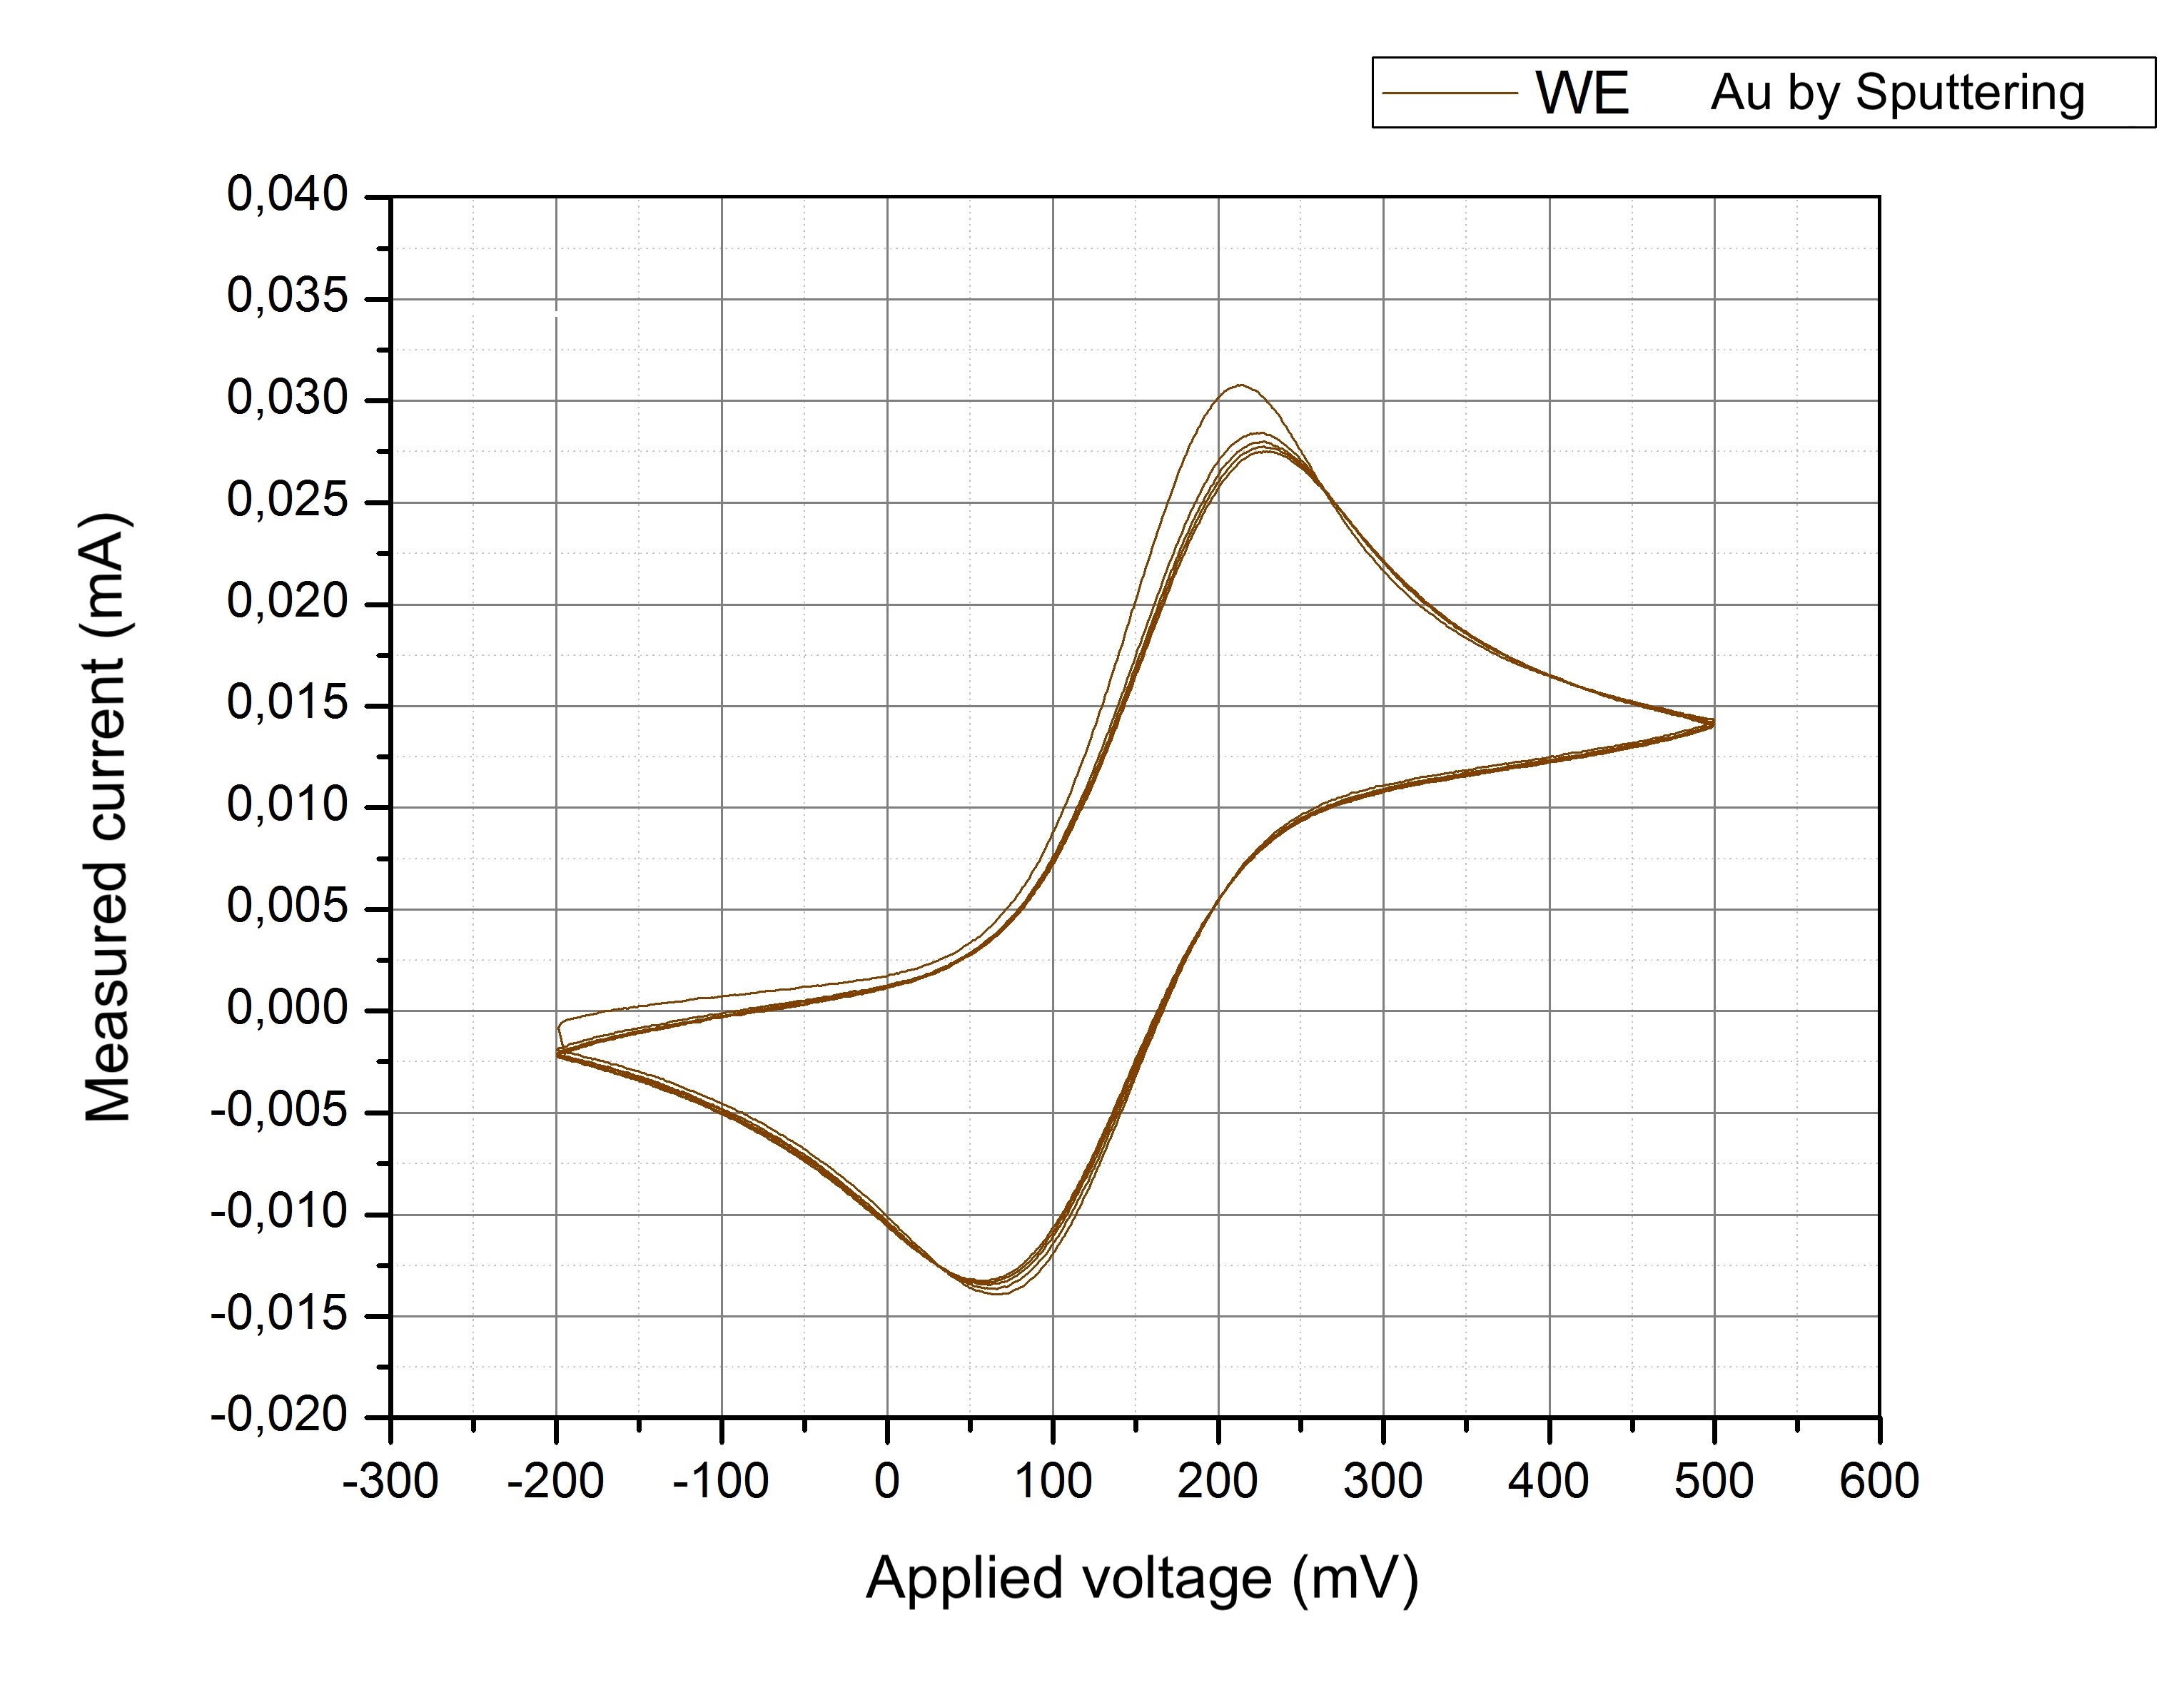
\includegraphics[width=0.8\textwidth]{Figures/Figura_EQ_Oro_Sputtering_1mm}
  \caption{Cyclic voltammetry with gold electrode obtained by Sputtering.}
  \label{fig:Figura_EQ_Oro_Sputtering_1mm}
\end{figure}

As a second measurement, it was decided to observe the behavior of the electrochemical probes on a carbon electrode (Figure ~\ref{fig:Figura_EQ_Carbono}), thus having the two curves that would overlap when testing a carbon electrode covered by the ink of gold nanoparticles.

\begin{figure}[H]
  \centering
    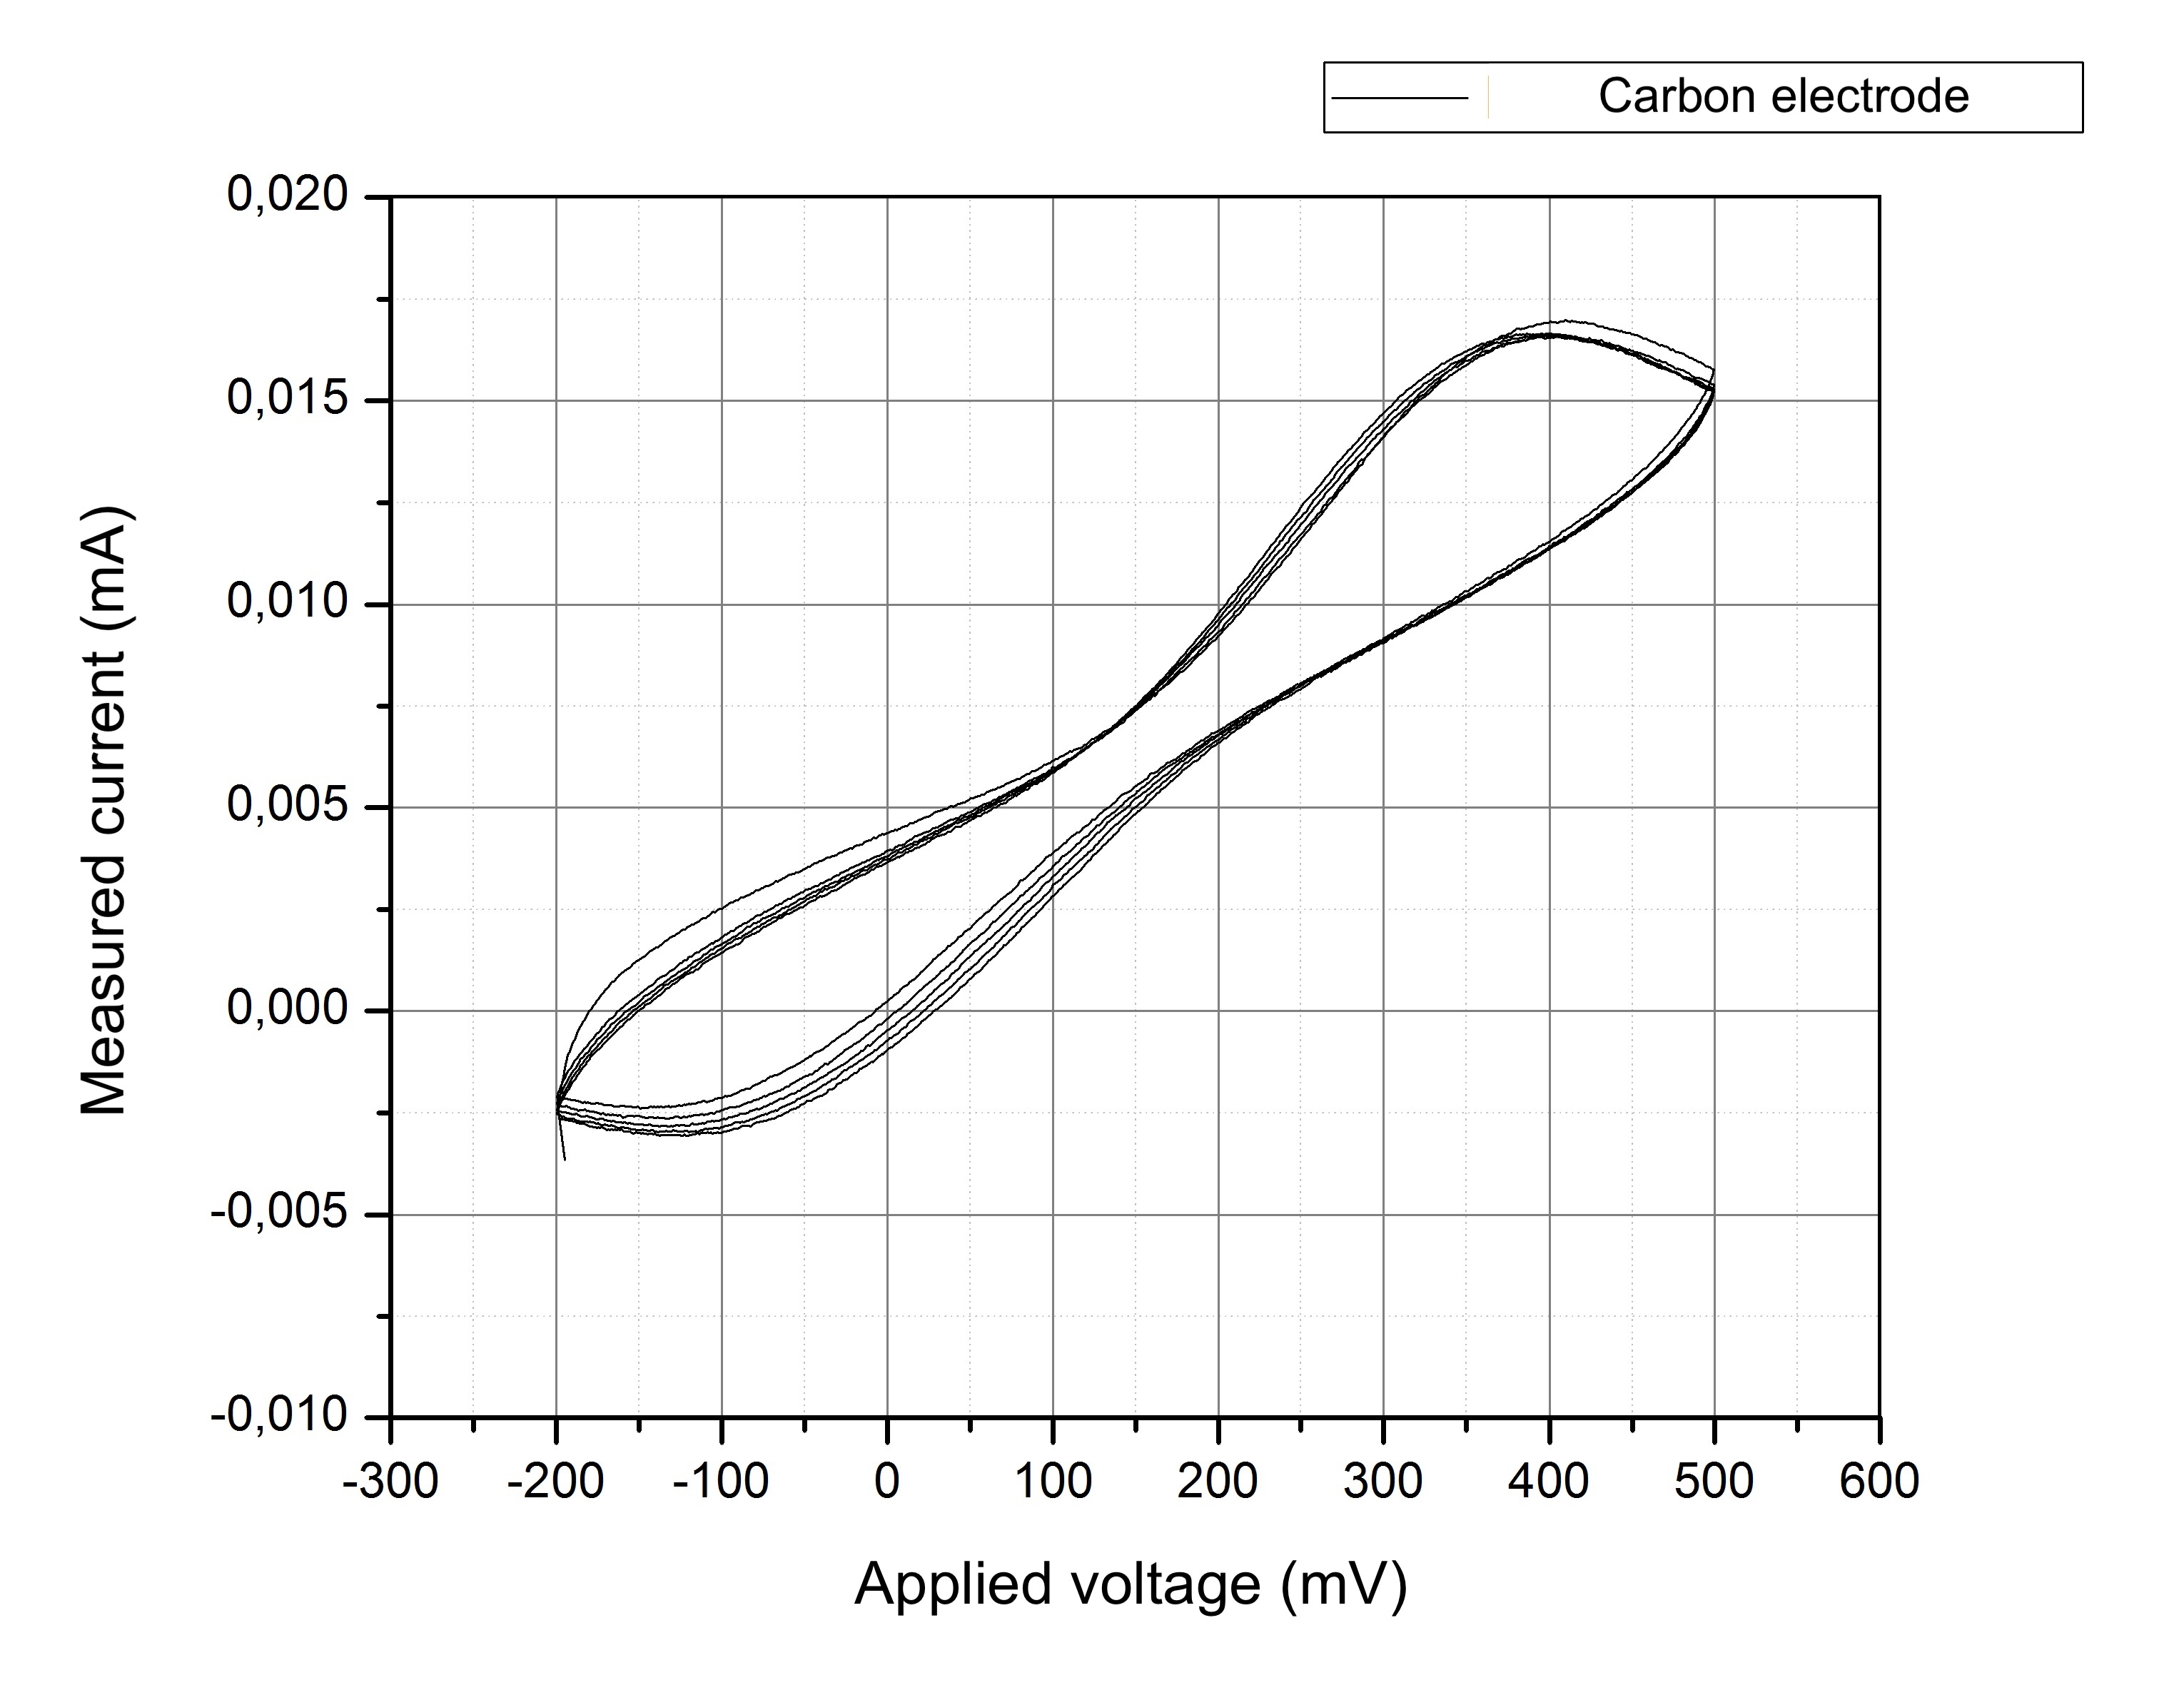
\includegraphics[width=0.8\textwidth]{Figures/Figura_EQ_Carbono}
  \caption{Cyclic voltammetry with carbon electrode.}
  \label{fig:Figura_EQ_Carbono}
\end{figure}
The next electrochemical measurement was performed on a carbon electrode coated with two layers of gold nanoparticle ink with 1 mm (Figure ~\ref{fig:Figura_EQ_Oro_Inkjet_Ambos} (a)) and 1.1 mm (Figure ~\ref{fig:Figura_EQ_Oro_Inkjet_Ambos} (b)) in diameter.

Comparing the result of the cyclical voltammetric curve of the electrochemical cell with gold \emph{WE} deposited by \textit{Sputtering} with the \emph{WE} with gold nanoparticles ink (Figure ~\ref{fig:Figura_EQ_Sputt_2-Inkjet}), the similarity is observed maintaining the current peaks corresponding to the gold.

\begin{figure}[H]
  \centering
    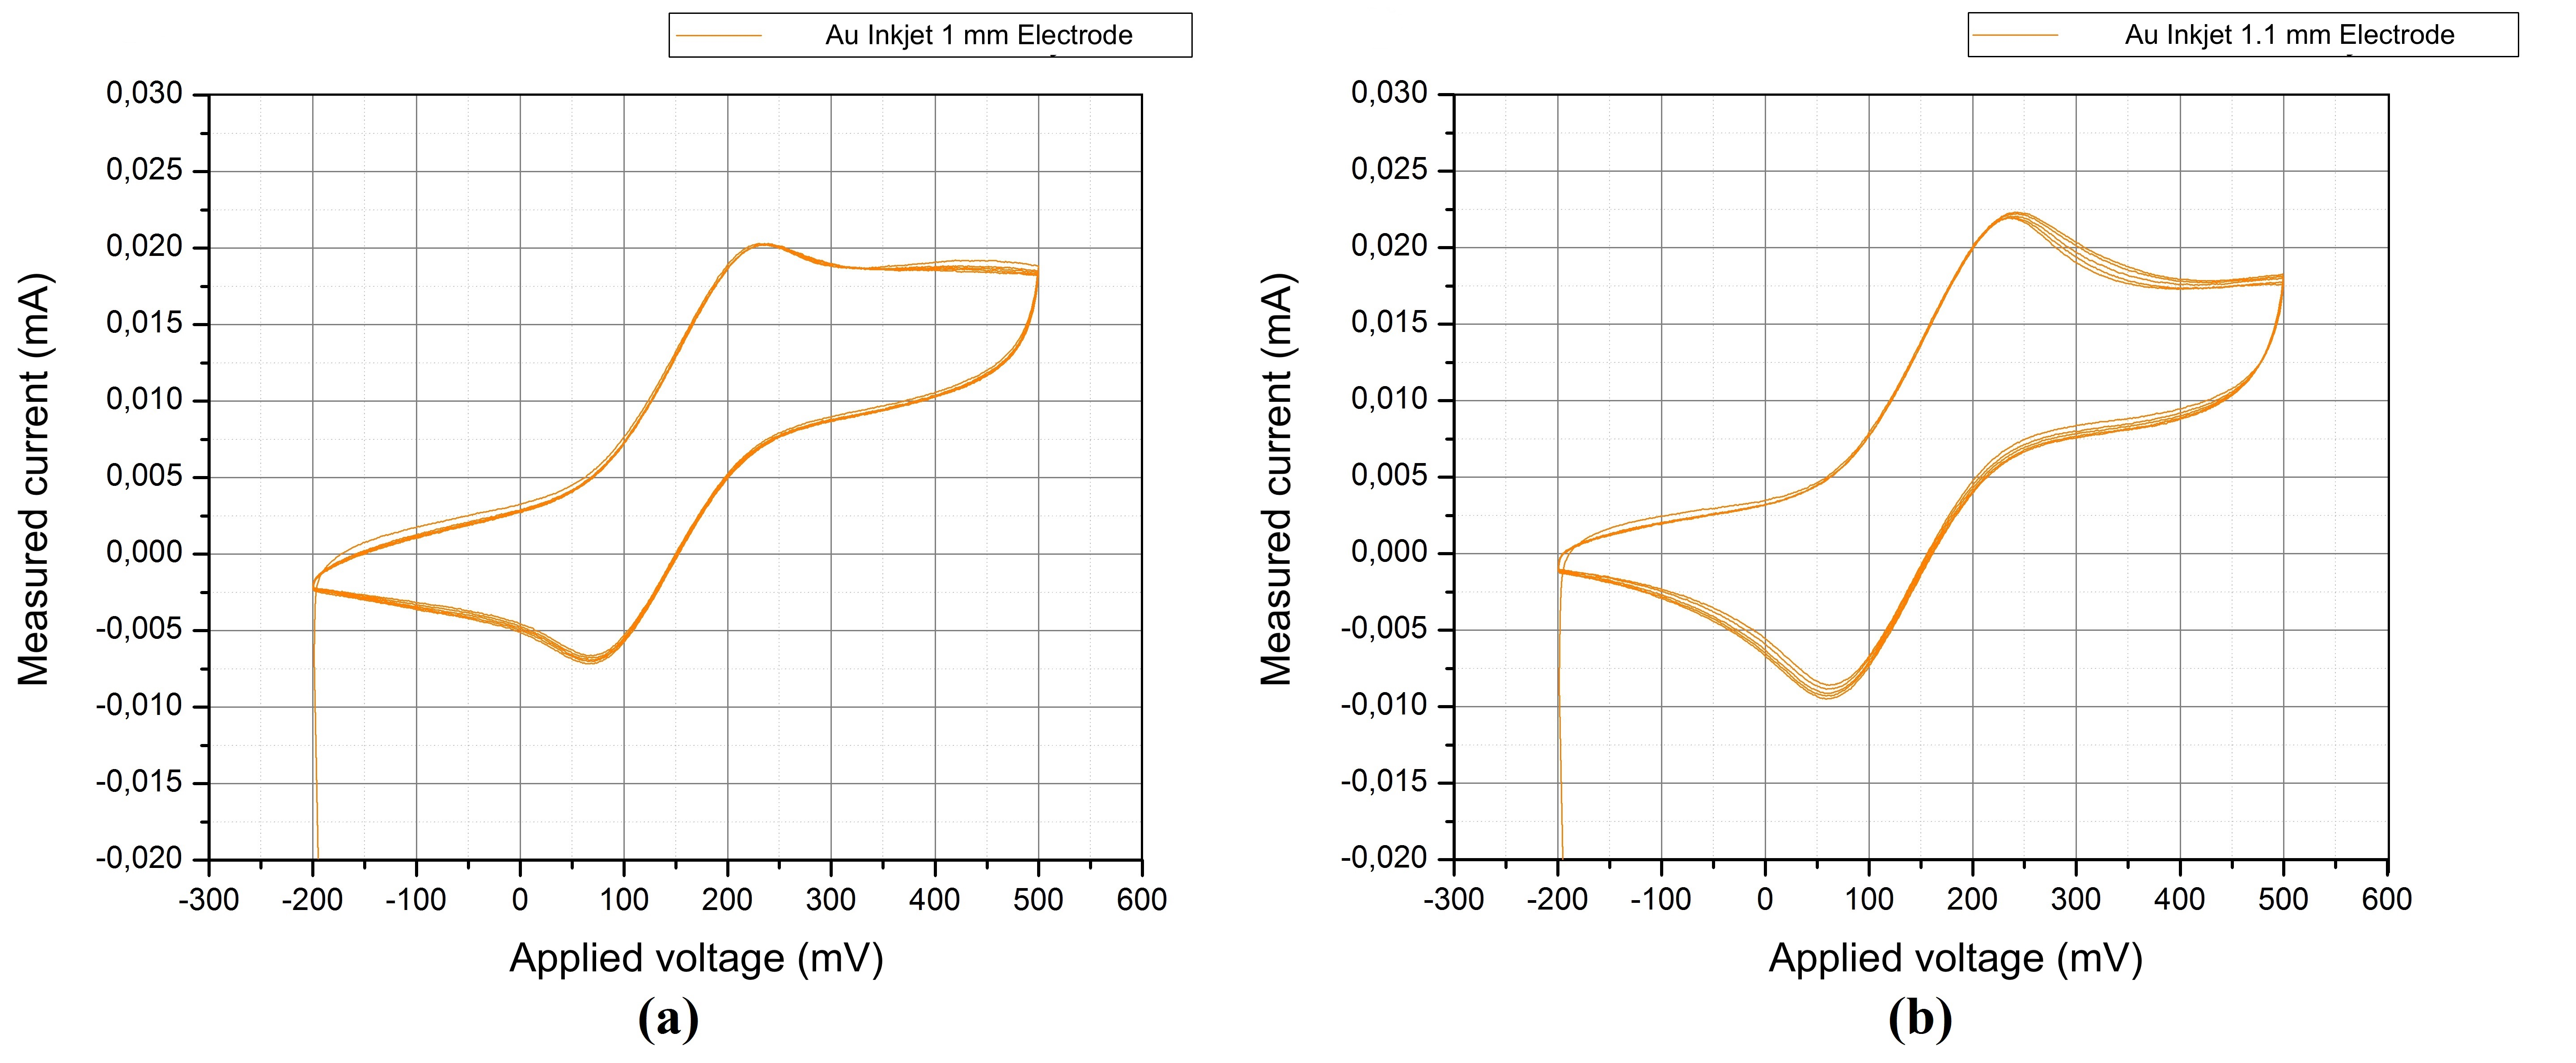
\includegraphics[width=1\textwidth]{Figures/Figura_EQ_Oro_Inkjet_Ambos}
  \caption{Cyclic voltammetry with carbon \emph{WE} coated with gold nanoparticles ink of different diameters: (a) 1 mm; (b) 1.1 mm.}
  \label{fig:Figura_EQ_Oro_Inkjet_Ambos}
\end{figure}

\begin{figure}[H]
  \centering
    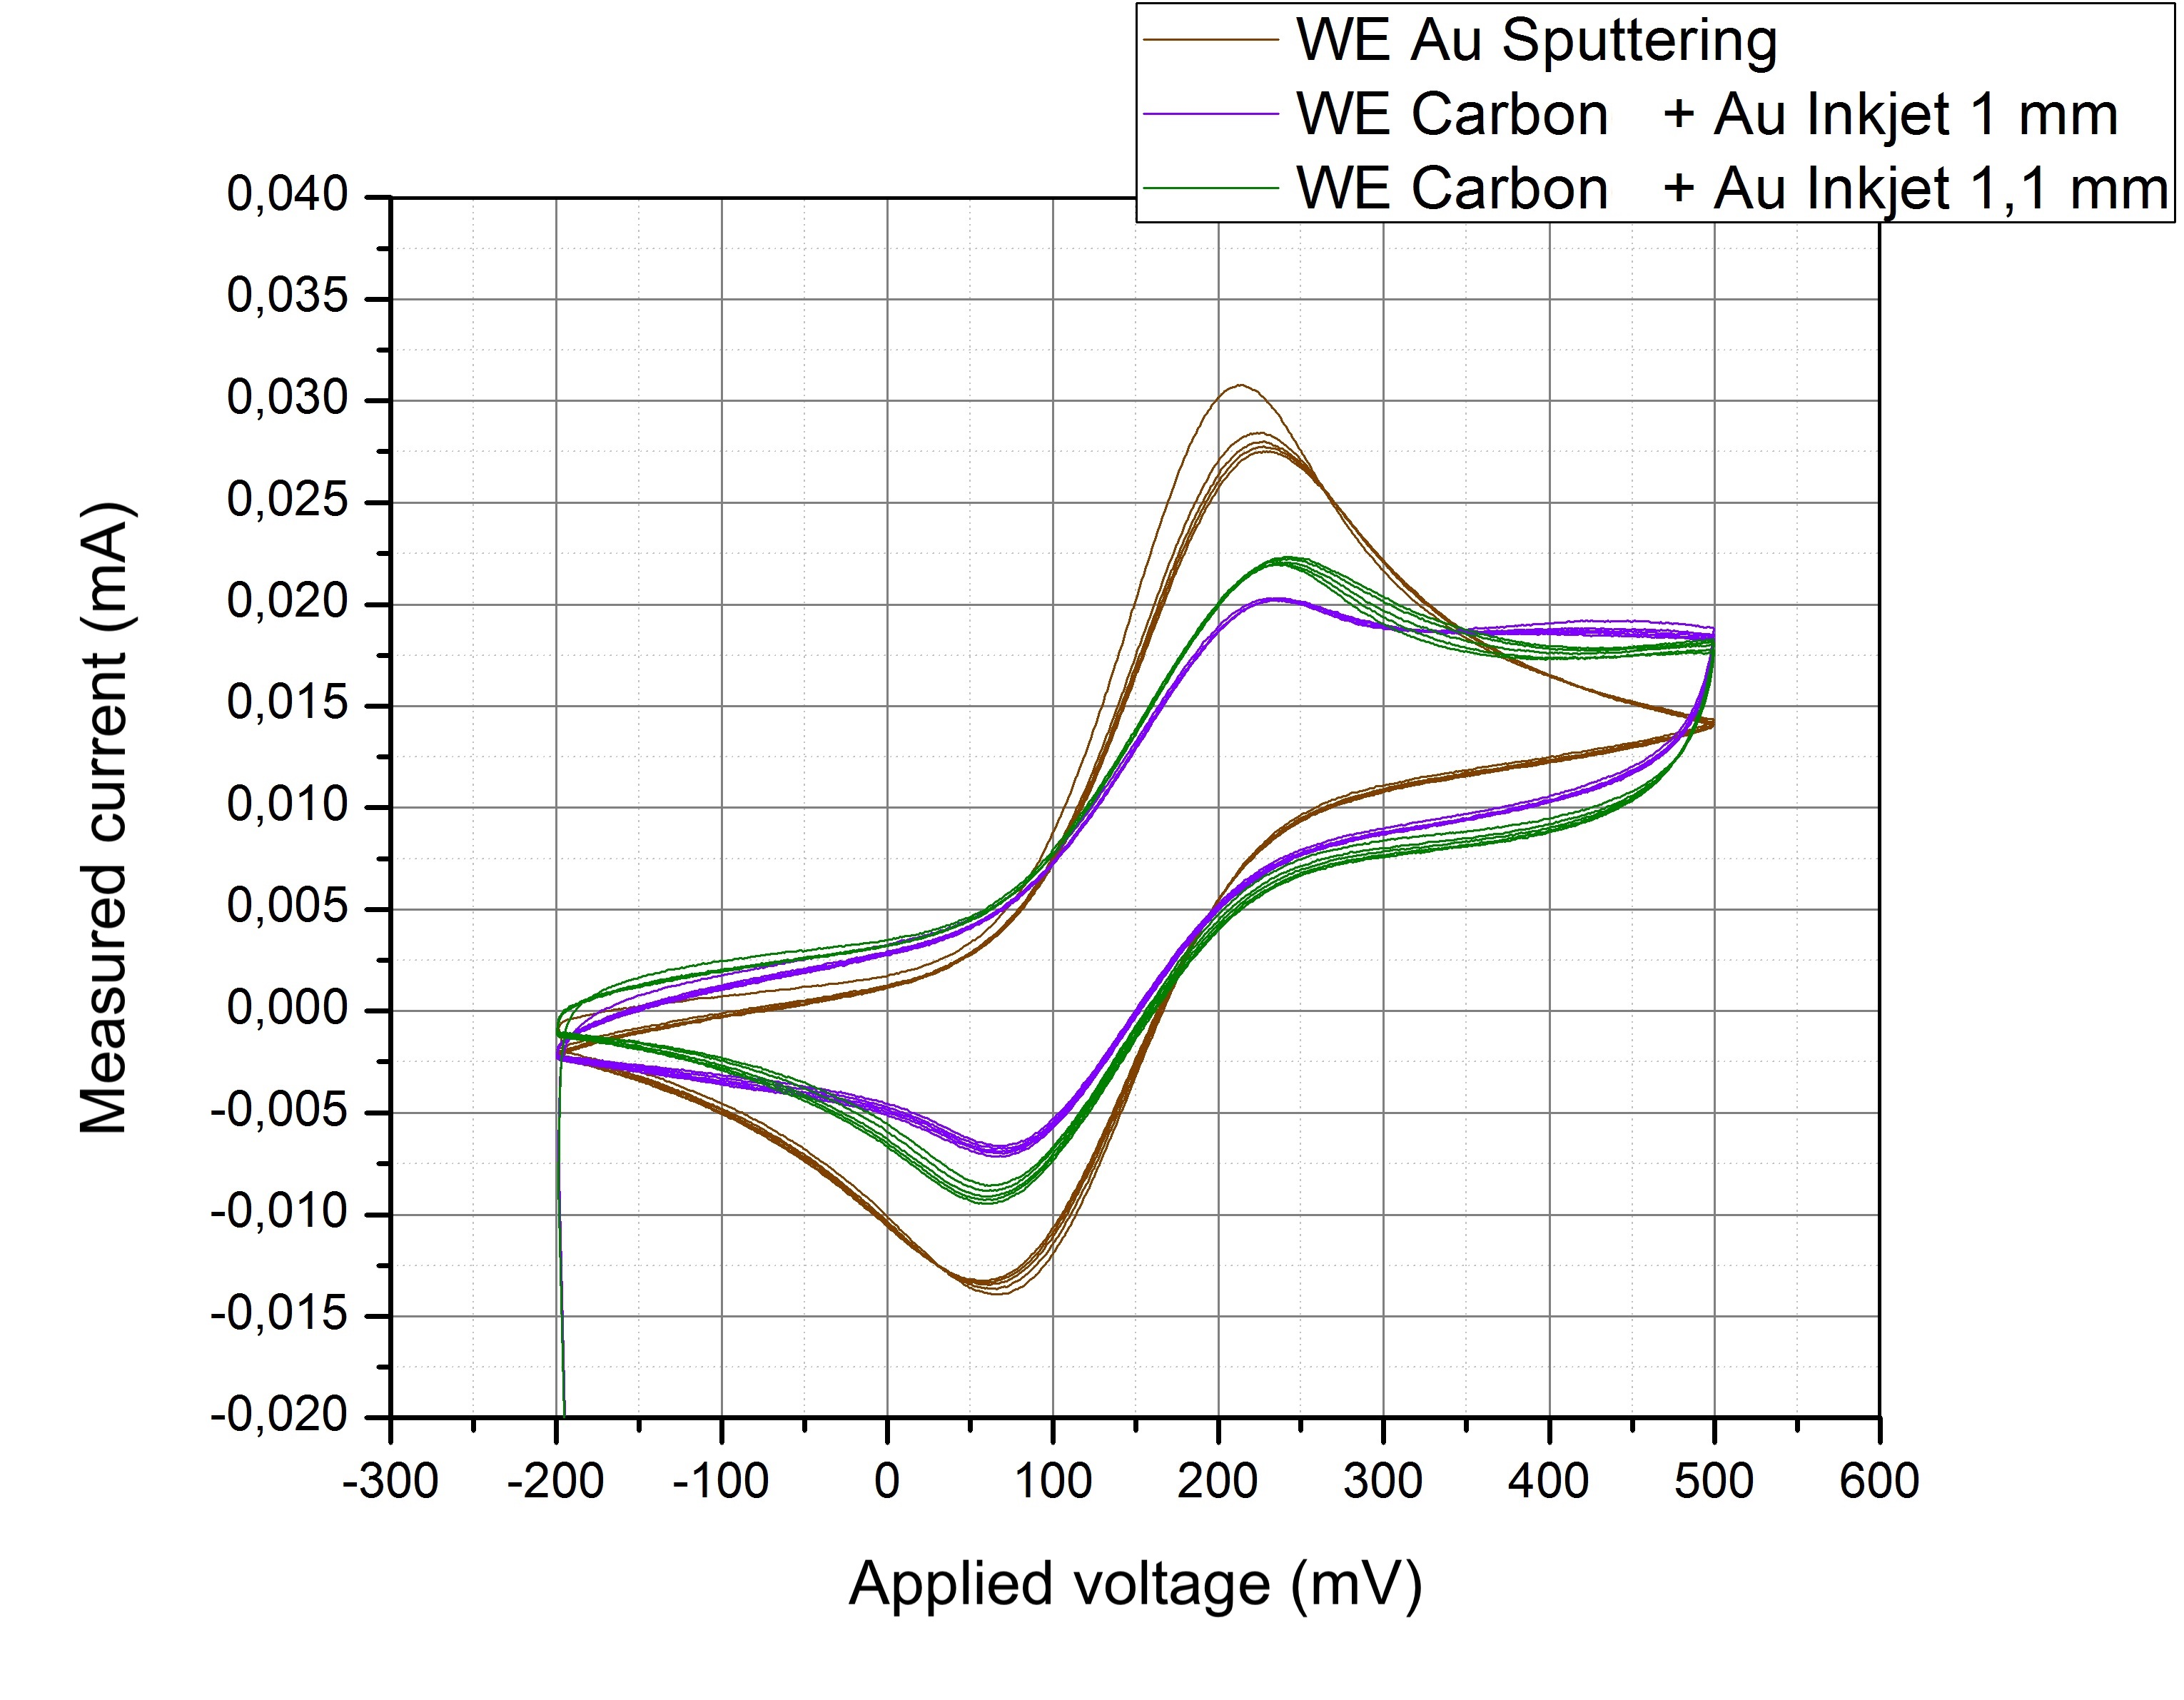
\includegraphics[width=0.8\textwidth]{Figures/Figura_EQ_Sputt_2-Inkjet}
  \caption{Comparison of cyclic voltammetries of electrochemical cells with gold \emph{WE} deposited by \textit{Sputtering} and with carbon \emph{WE} with gold nanoparticles ink.}
  \label{fig:Figura_EQ_Sputt_2-Inkjet}
\end{figure}

The increase of intensity in the electrodes with gold \textit{inkjet} printing is due to the presence of carbon underneath it, as can be verified by overlapping the previous curves with that of pure carbon (Figure ~\ref{fig:Figura_EQ_Oro_Inkjet_Ambos}) and also, the increase in the effective area of the \emph{WE} due to the difference in roughness between the gold deposited by \textit{sputtering}  and the ink of gold nanoparticles printed by \textit{inkjet}.

\begin{figure}[H]
  \centering
    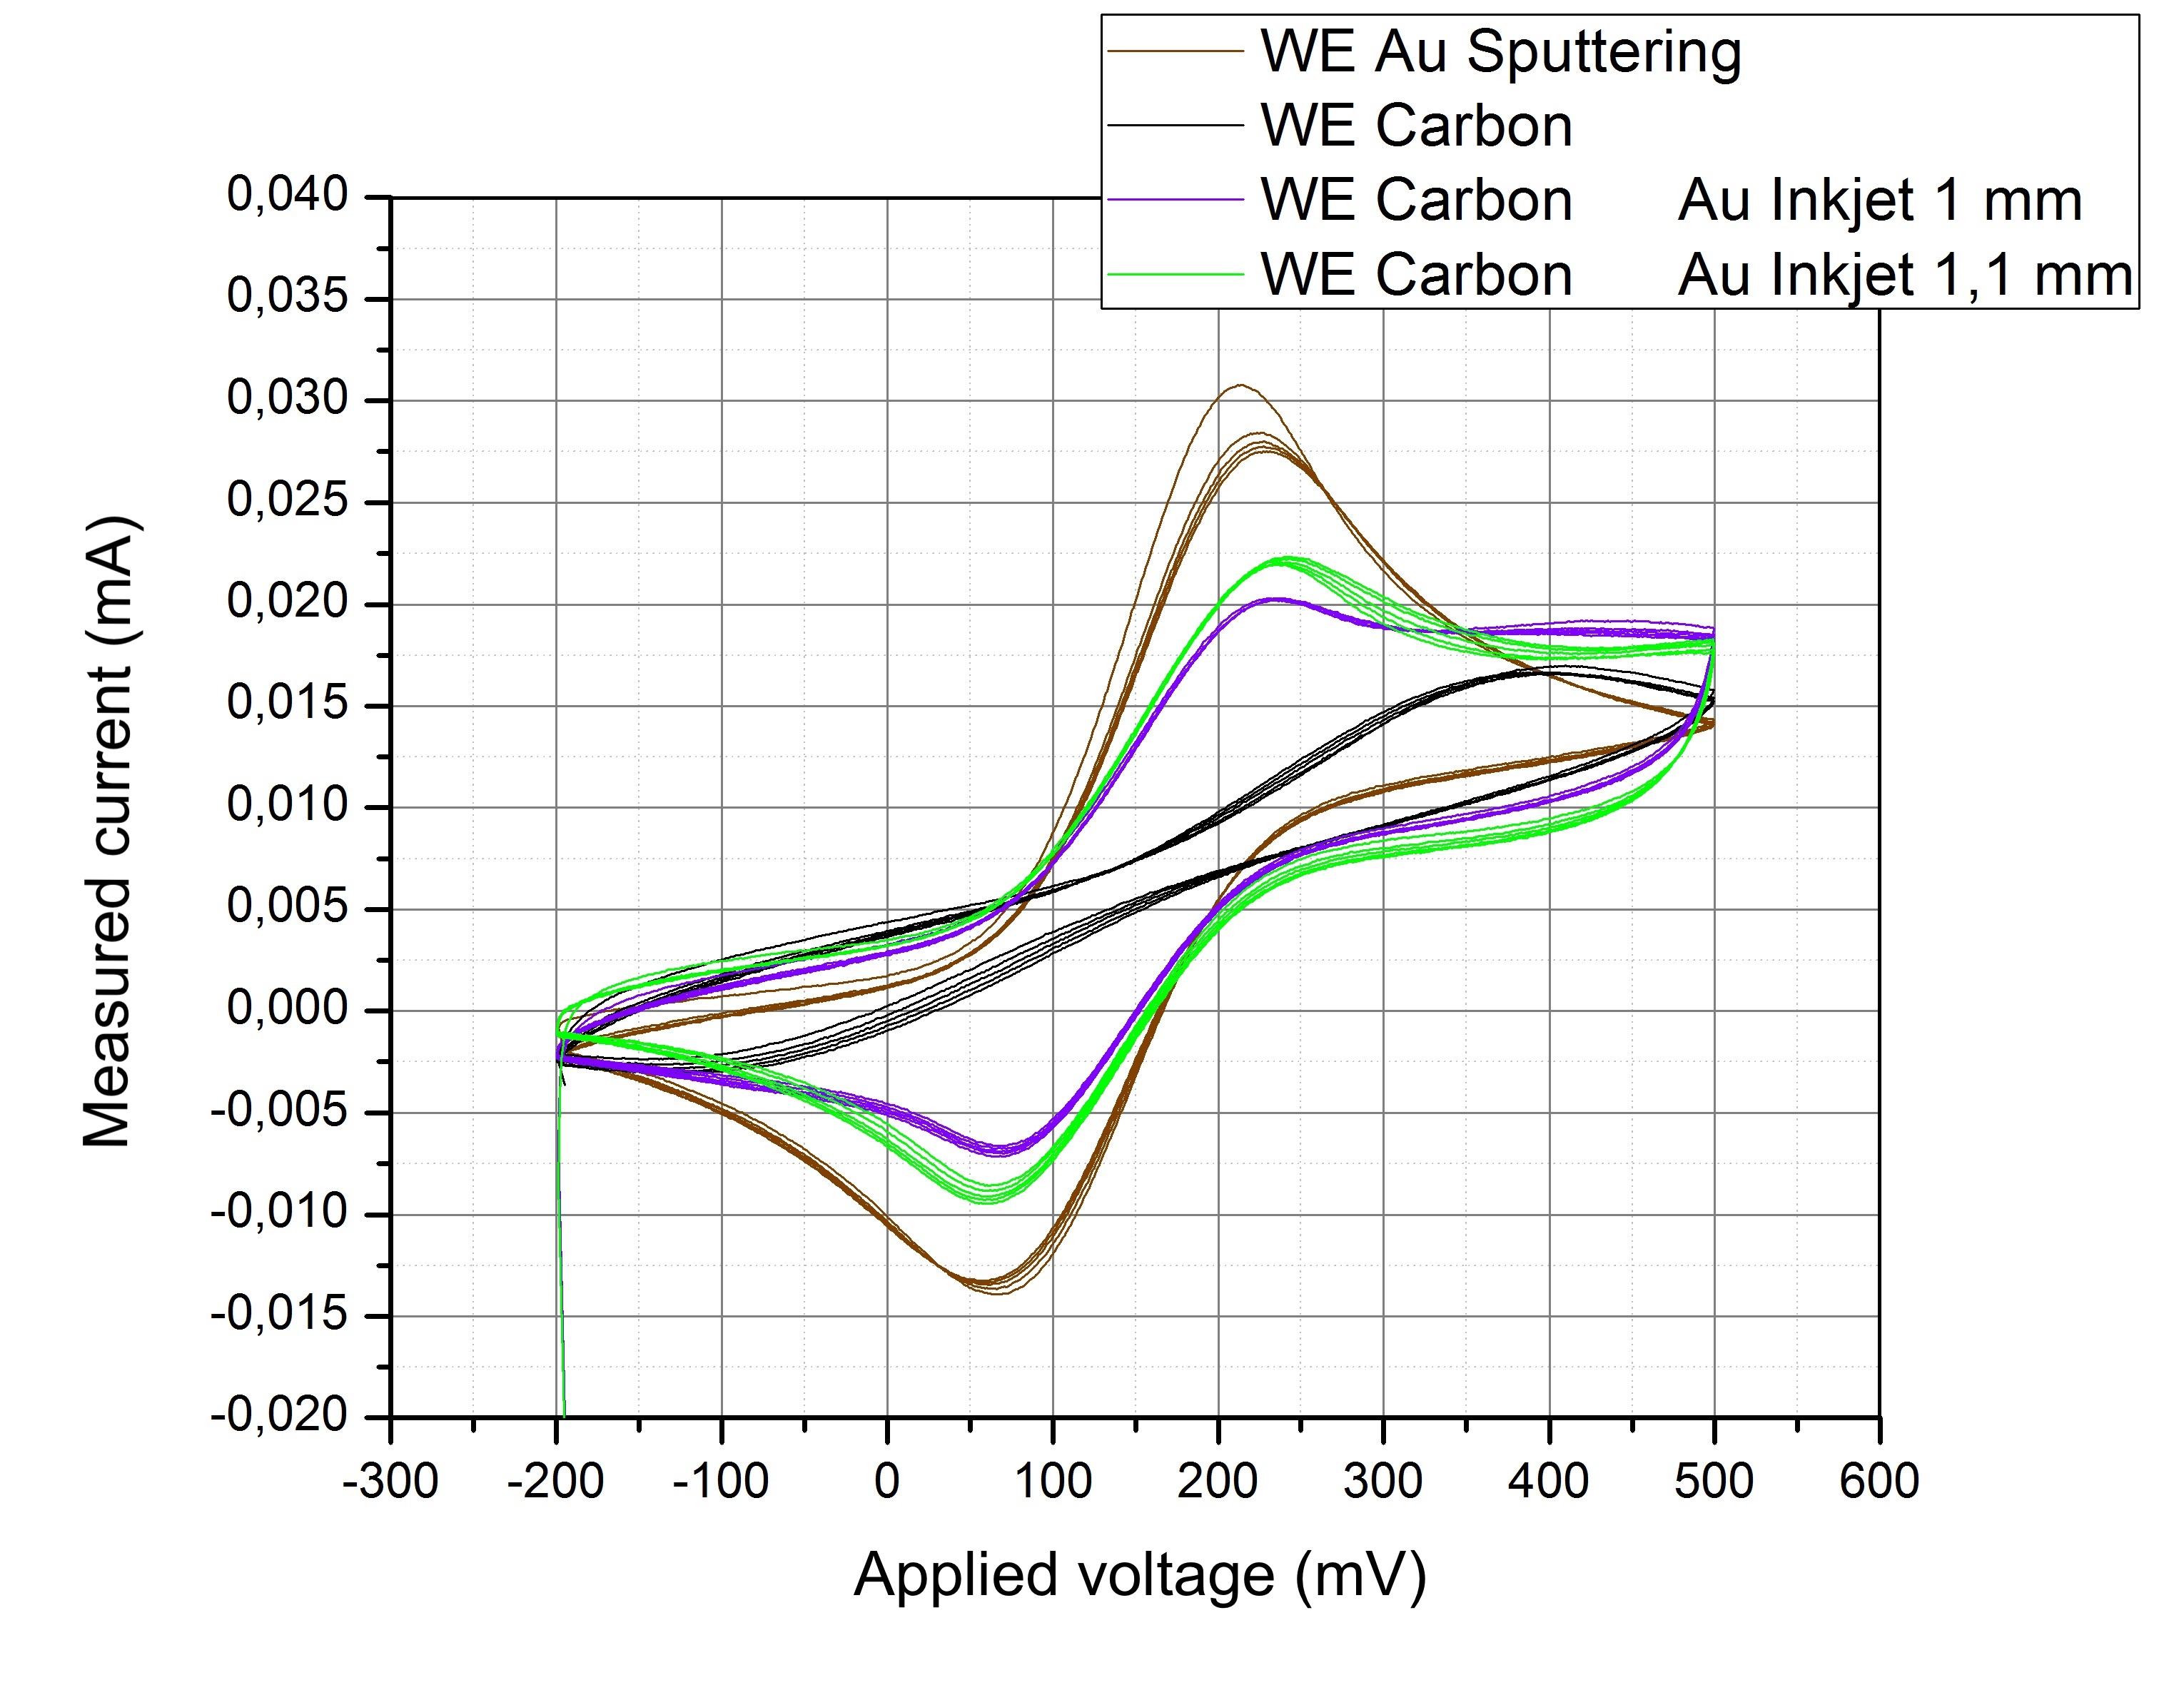
\includegraphics[width=0.8\textwidth]{Figures/Figura_EQ_Sptt_AuInkjet_Carbono_Valox}
  \caption{Overlapping \emph{WE} with gold deposited by \textit{Sputtering}, carbon \emph{WE} and carbon \emph{WE} with gold nanoparticles ink.}
  \label{fig:Figura_EQ_Sptt_AuInkjet_Carbono_Valox}
\end{figure}

To have comparisons of the nanoparticles ink on different substrates, measurements of the \textit{Inkjet} printed ink were made on Valox, PET and cellulose pulp sheet (Figure ~\ref{fig:Figura_EQ_Inkjet_Valox_PET_Papel}).

\begin{figure}[H]
  \centering
    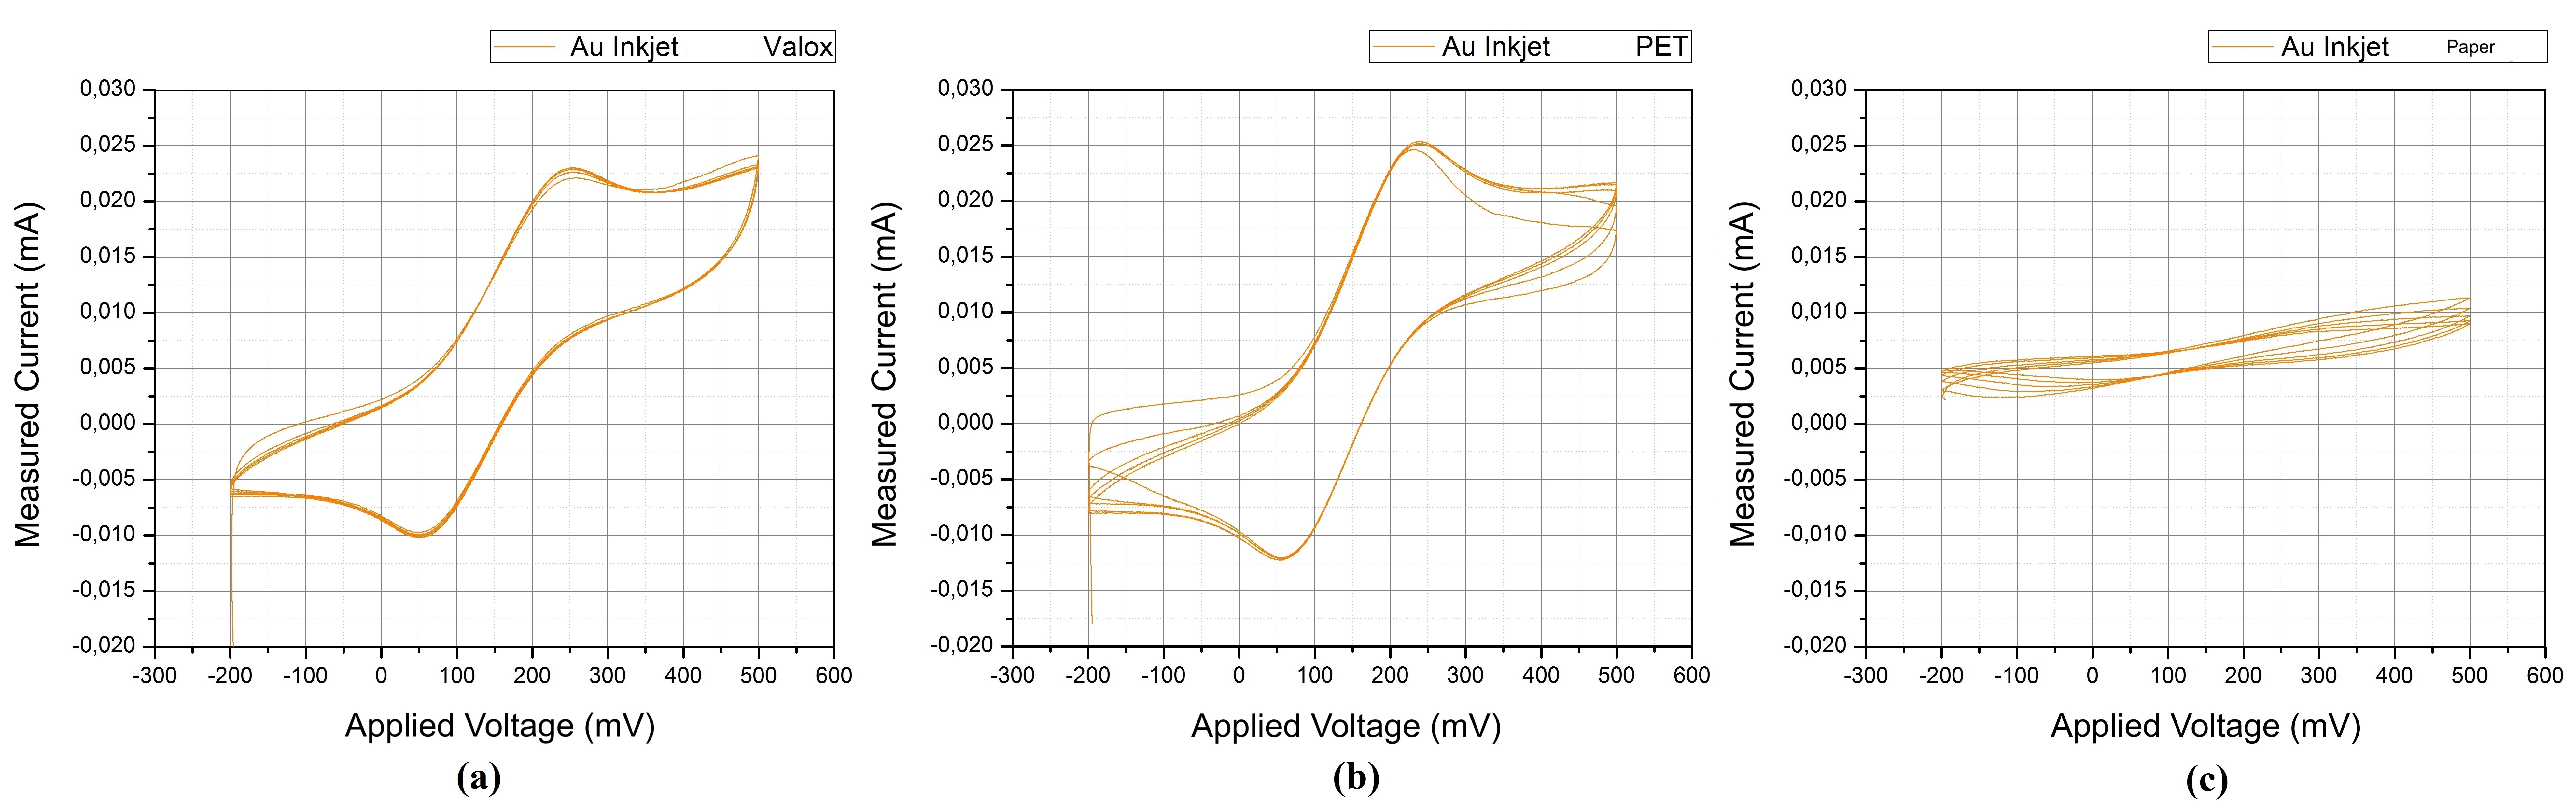
\includegraphics[width=1\textwidth]{Figures/Figura_EQ_Inkjet_Valox_PET_Papel}
  \caption{Results of cyclic voltammetry on \textit{inkjet} printing of ink with gold nanoparticles on: (a) Valox; (b) PET and (c) Paper.}
  \label{fig:Figura_EQ_Inkjet_Valox_PET_Papel}
\end{figure}

The comparable results obtained between the gold deposited by \textit{Sputtering} and the \textit{Inkjet} printing on smooth substrate (PET) stands out (Figure ~\ref{fig:Figura_EQ_Sputt_Inkjet_PET}).

\begin{figure}[H]
  \centering
    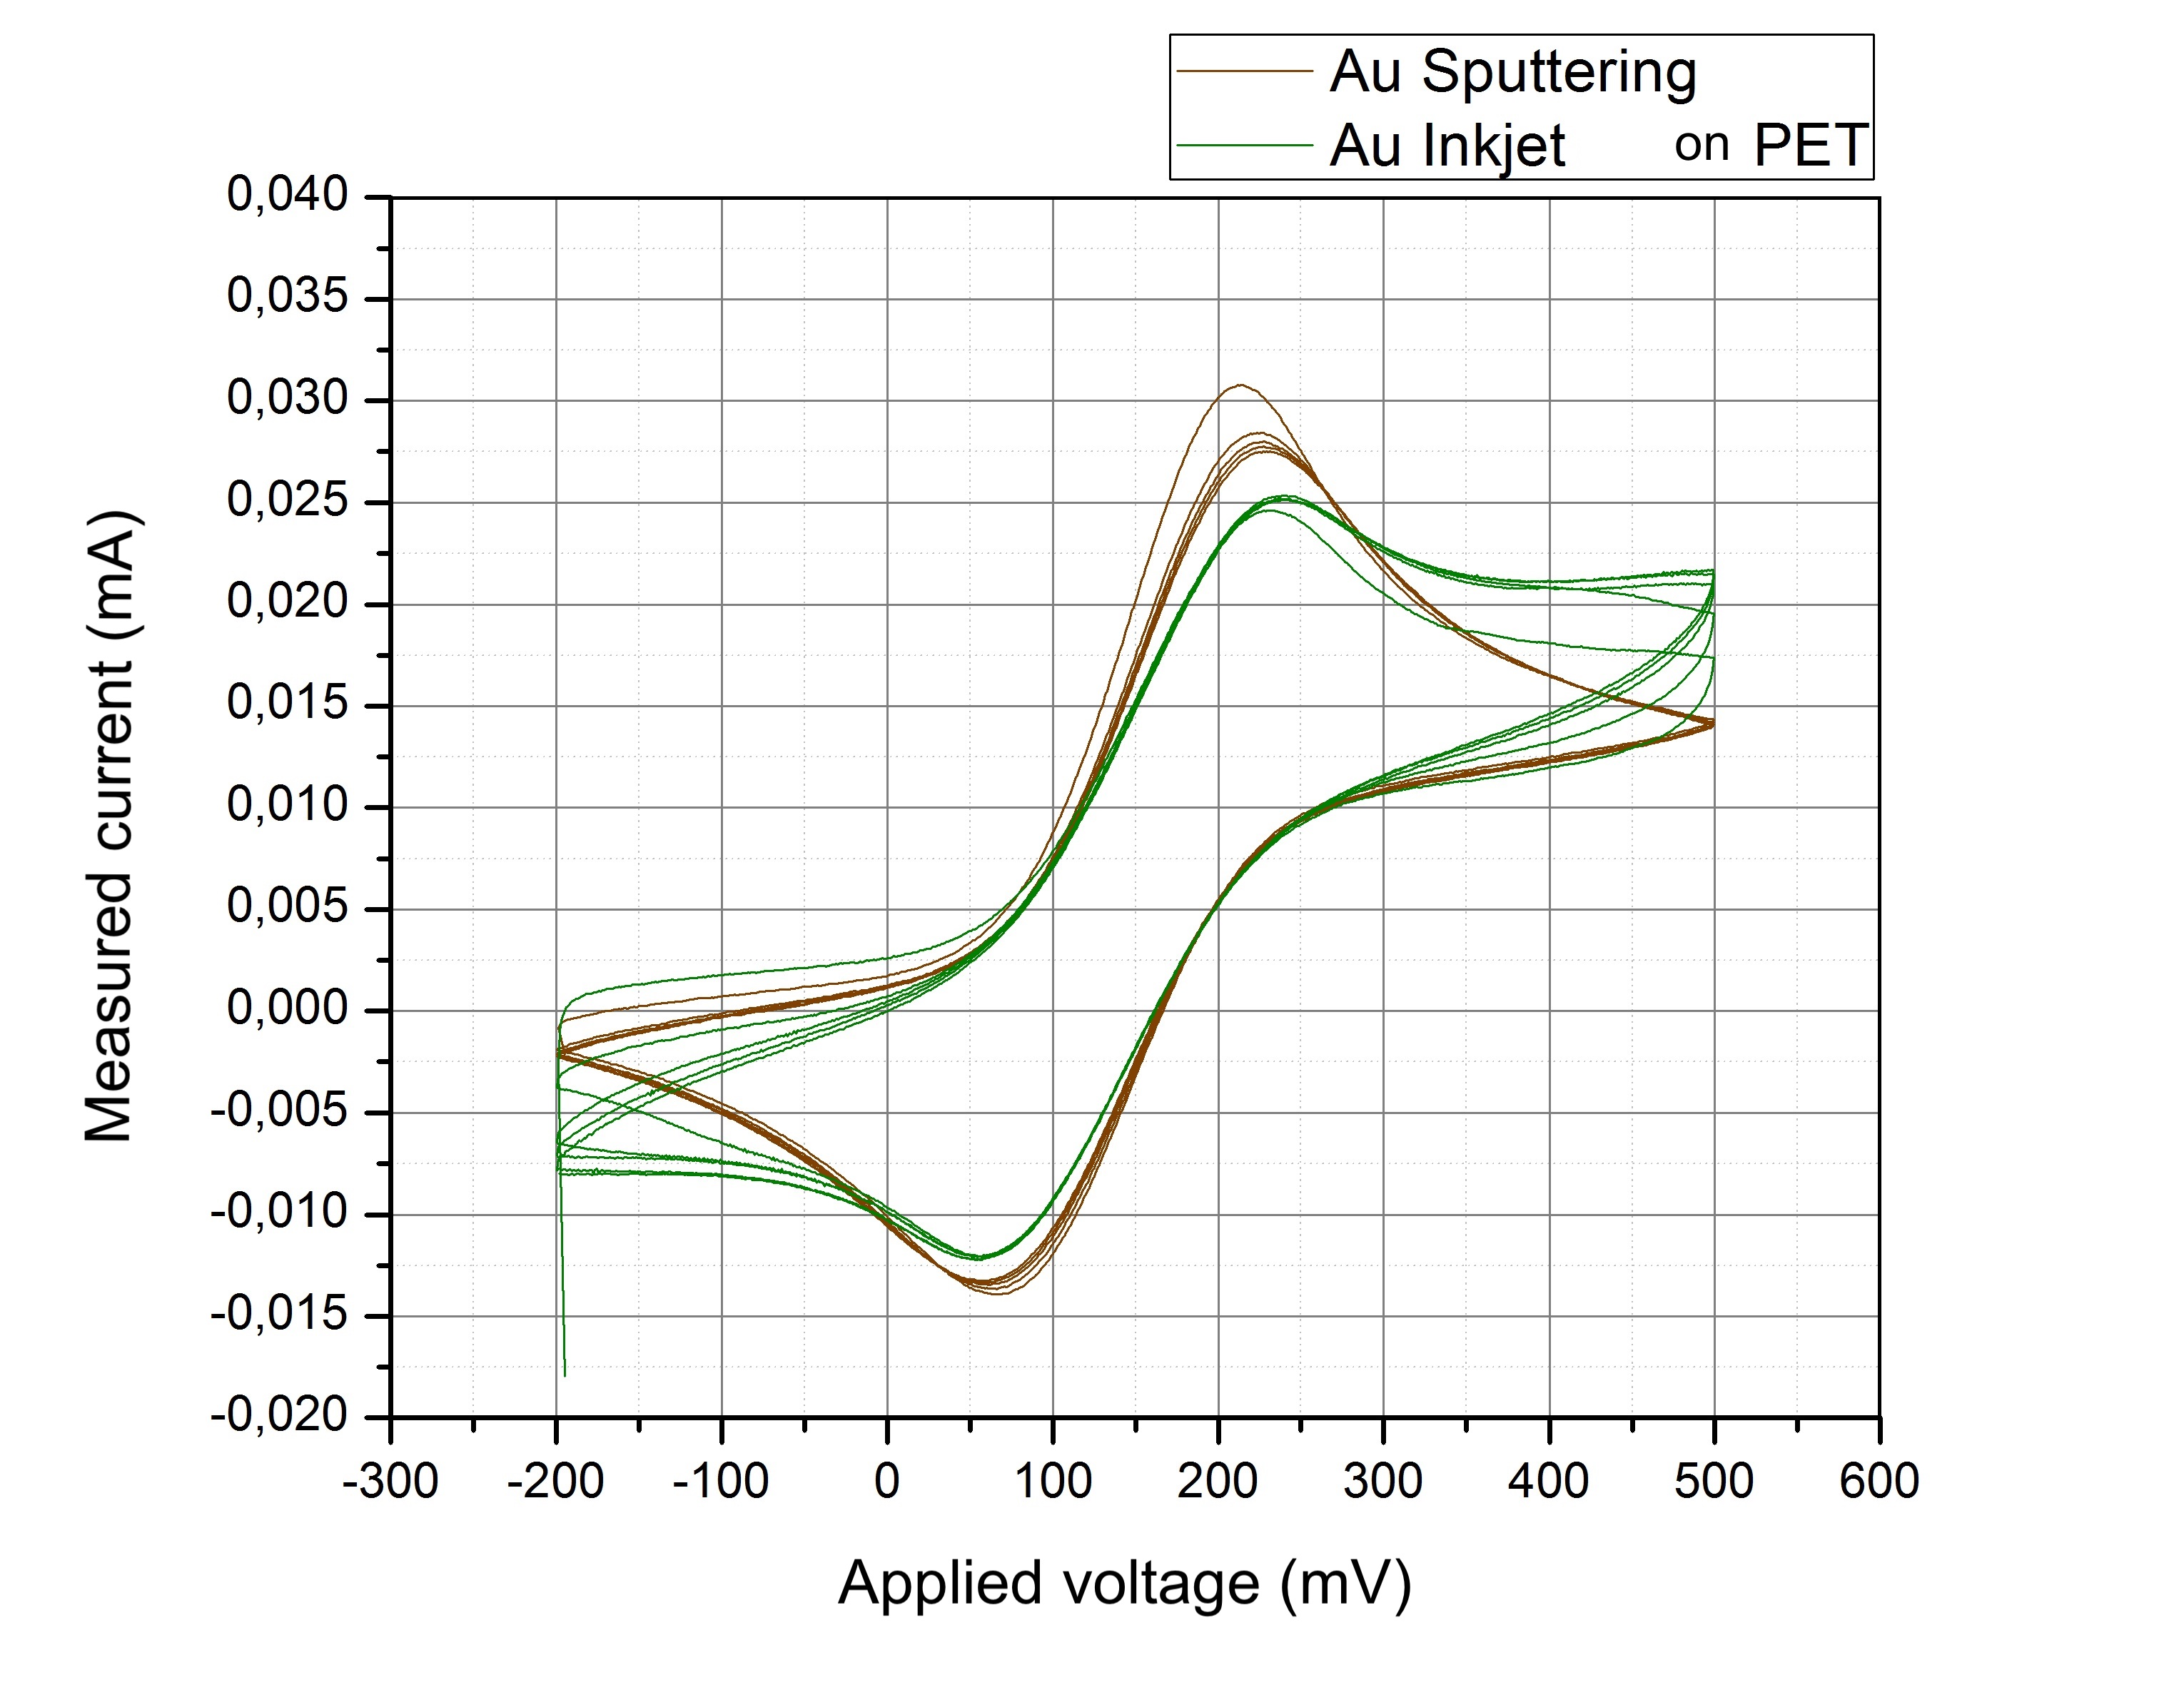
\includegraphics[width=0.8\textwidth]{Figures/Figura_EQ_Sputt_Inkjet_PET}
  \caption{Comparison of cyclic voltammetry on \emph{WE} of gold deposited by \textit{Sputtering} and \textit{inkjet} printing of ink with gold nanoparticles on PET.}
  \label{fig:Figura_EQ_Sputt_Inkjet_PET}
\end{figure}